\paragraph{}
Ze względu na architekturę aplikacji, klasy używane na CPU oddzielone są od klas karty graficznej. Oczywiście te drugie są klasami jedynie logicznie - ze względu na konieczność używania języka C w kodzie dla GPU. Ponieważ jednak obiekty są wygodną abstrakcją, będziemy z niej korzystać w całym programie.

\subsubsection{Klasy GPU}

\begin{figure}[h]
	\centering
	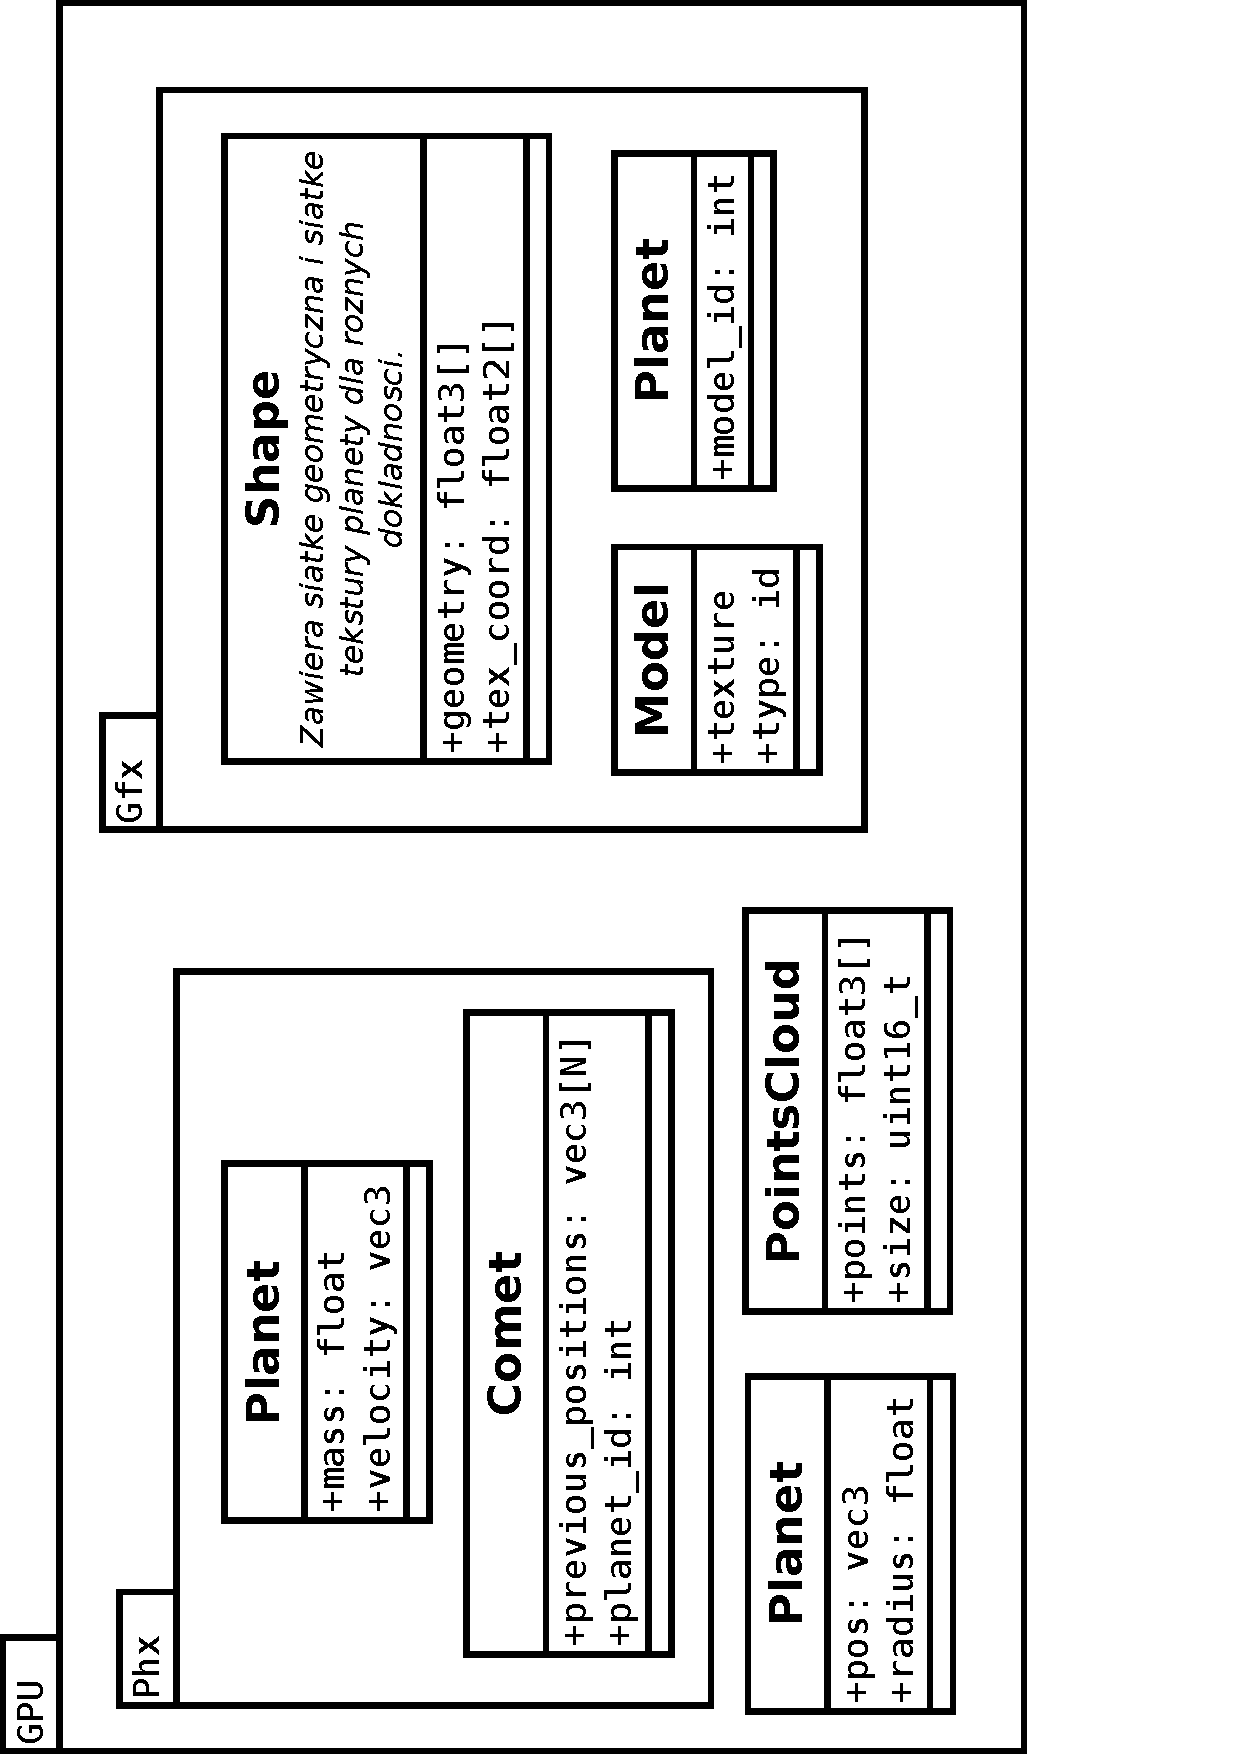
\includegraphics[angle=270,width=0.8\textwidth]{class_gpu.pdf}
	\caption{Diagram klas dla GPU}
	\label{fig:class_gpu}
\end{figure}

\paragraph{}
Struktury, z których będziemy korzystać na karcie graficznej, określone są na rysunku \ref{fig:class_gpu}. Ponieważ karta graficzna służy nam zarówno do wyświetlania danych, jak i do ich przetwarzania, wydzielone są na nim dwie przestrzenie nazw. Są to:
\begin{itemize}
	\item{Phx - do operacji fizycznych}
	\item{Gfx - do operacji graficznych}
\end{itemize}

\paragraph{}
Ponadto istnieje kilka struktur wspólnych dla obu częsci.

\begin{description}
\item{\bf GPU::Planet} zawiera informacje, z których korzystaja zarówno wyświetlanie jak i fizyka. Jest to położenie planety oraz jej promień.
\item{\bf GPU::PointsCloud} reprezentuje chmurę cząstek - jest ona obliczana dla każdej widocznej komety przez moduł fizyczny.
\end{description}

\paragraph{}

Operacje fizyczne odbywać się będą z wykorzystaniem dwóch dodatkowych struktur.

\begin{description}
\item{\bf GPU::Phx::Planet} to dodatkowe informacje o każdej planecie, które są potrzebne jedynie silnikowi fizycznemu. Należą do nich prędkość oraz masa.
\item{\bf GPU::Phx::Comet} stanowi dodatkową informację o planecie. Struktura ta istnieje tylko dla obiektów będących kometami. Zawiera kilka ostatnich pozycji oraz identyfikator planety.
\end{description}

\paragraph{}

Do wyświetlenia planet konieczne będą informacje o teksturach, oraz o siatkach każdej z planet.

\begin{description}
\item{\bf GPU::Gfx::Planet} zawiera indeks modelu, czyli wyglądu planetu. Dwie planety mogą mieć ten sam model.
\item{\bf GPU::Gfx::Model} definiuje konkretny wygląd. Na tym poziomie będziemy rozróżniać zwykłe planety od gwiazd i komet.
\item{\bf GPU::Gfx::Shape} agreguje informację o siatce planety w 3D oraz odpowiadającej jej siatce na dwuwymiarowej teksturze.
\end{description}

\subsubsection{Klasy CPU}

\begin{figure}[ht!]
	\centering
	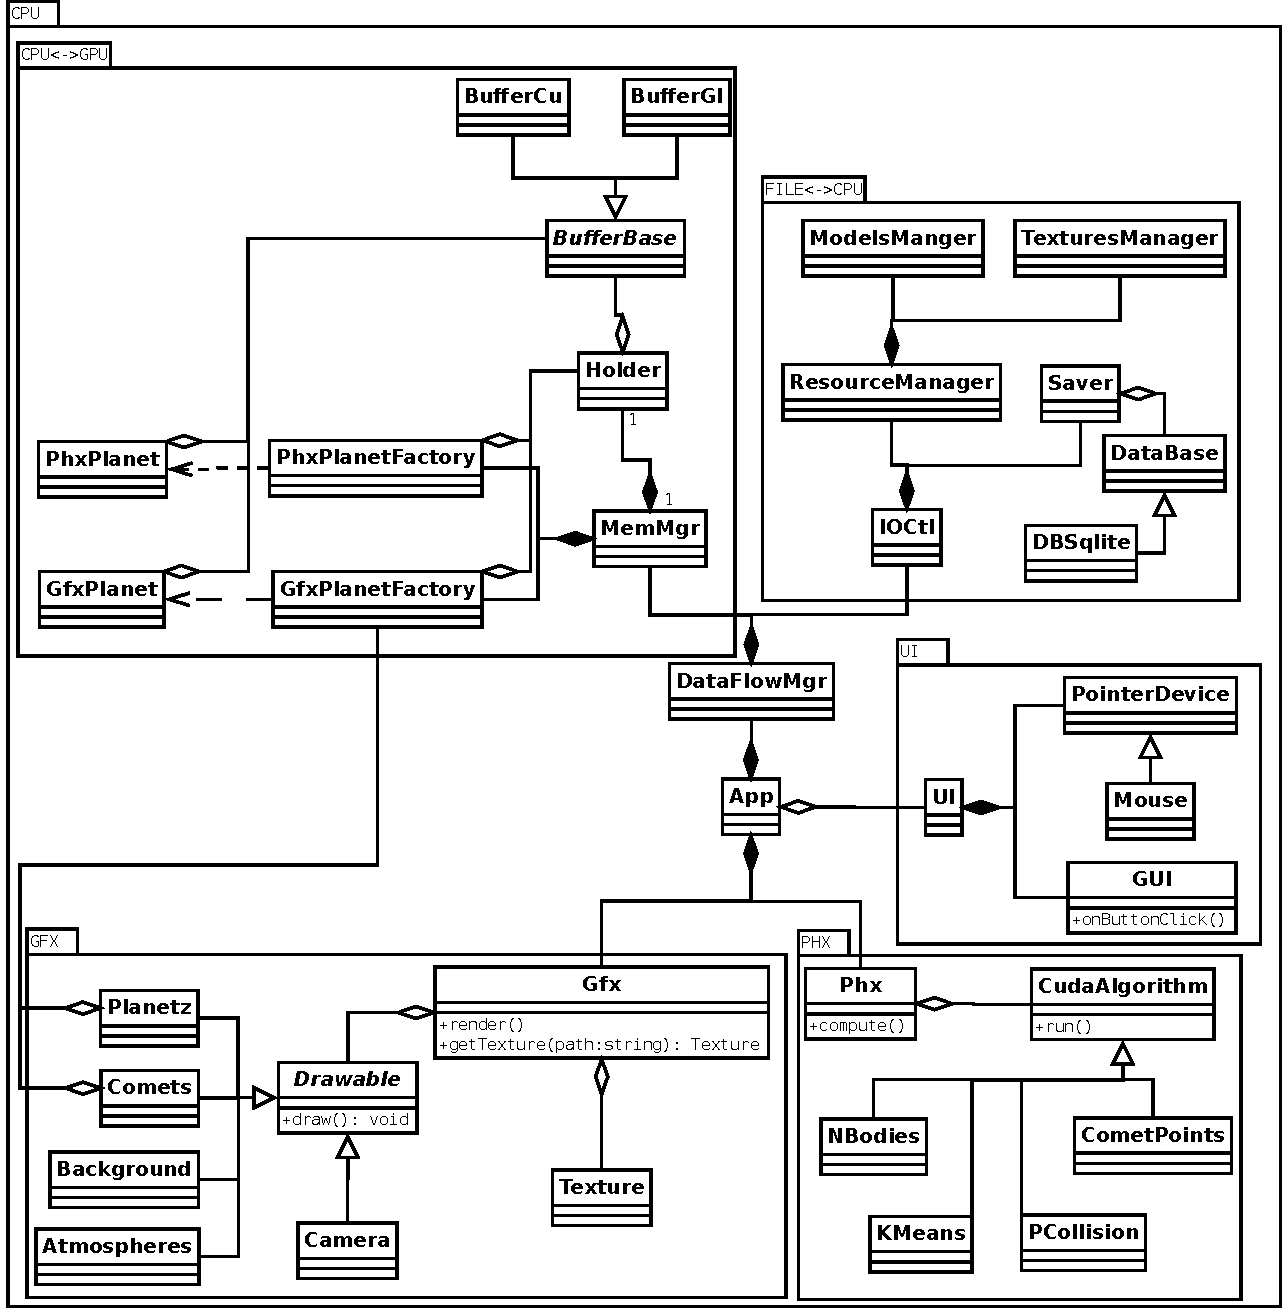
\includegraphics[angle=0,width=\textwidth]{class_cpu.pdf}
	\caption{Diagram klas dla CPU}
	\label{fig:class_cpu}
\end{figure}

\paragraph{}
Ta część klas przełoży się bezpośrednio na klasy znane z c++. Diagram klas znajduje się na rysunku \ref{fig:class_cpu}.

\begin{description}
\item{\bf CPU::App} jest główną klasą, zarządzającą obiektami GFX, PHX, DataFlowMgr oraz UI. Tworzy je ona na początku działania programu.
\item{\bf CPU::DataFlowMgr} wykonuje wszystkie przepływy danych - pomiędzy RAM karty graficznej, RAM komputera oraz dyskiem twardym.
\item{}
\item{\bf CPU::PHX::Phx} uruchamia kernel'e CUDA, które przeprowadzają wszystkie obliczenia fizyczne.
\item{}
\item{\bf CPU::GFX::Gfx} odpowiada za wyświetlanie wszystkich obiektów obecnych w przestrzeni 3D. Korzysta przy tym z biblioteki OpenGL.
\item{\bf CPU::GFX::Drawable} abstrakcja dla wszystkich obiektów które chcą być wyświetlane.
\item{\bf CPU::GFX::Texture} obiekt tekstury, generowany przez klasę Gfx na podstawie bitmapy. Aby zapobiec zbędnemu ładowaniu tekstur, każda klasa która chce dostać taki obiekt, musi poprosić o niego klasę Gfx, która albo zwróci załadowaną teksturę, albo stworzy nowy obiekt tej klasy.
\item{\bf CPU::GFX::Planetz} obiekt wyświetlający wszystkie planety obecne na scenie.
\item{\bf CPU::GFX::Comets} obiekt wyświetlający wszystkie komety.
\item{\bf CPU::GFX::Background} wyświetla tło.
\item{\bf CPU::GFX::Atmospheres} klasa odpowiedzialna za wyświetlanie efektów atmosferycznych nad planetami.
\item{}
\item{\bf CPU::UI::UI} odpowiada za całość interakcji z użytkownikiem, czyli za obsługę zdarzeń myszki, klawiatury, oraz graficzny interfejs użytkownika.
\item{\bf CPU::UI::GUI}, czyli graficzny interfejs użytkownika. Składać sie na to będą okna oraz guziki zagnieżdżone w oknie głównym aplikacji.
\item{\bf CPU::UI::PointerDevice} abstrakcja dla wszystkich wejściowych urządzeń które mogą być wskaźnikami. W danej aplikacji będzie to najprawdopodobniej myszka, jednak takie podejście umożliwia dodanie obsługi takich peryferii jak dżojstiki czy kontrolery gier.
\item{\bf CPU::UI::Mouse} implementacja abstrakcji wskaźnika z użycie myszki.
\item{}
\item{\bf CPU::FILE2CPU::IOCtl} klasa bazowa modułu odpowiedzialnego za wczytywanie danych z plików do pamięci ram, oraz zapisywanie zmodyfikowanych danych do pliku.
\item{\bf CPU::FILE2CPU::ResourcesManager} klasa odpowiedzialna za zarządzenie zasobami aplikacji, takimi jak modele, tekstury i wszelkie inne dane przechowywane na dysku.
\item{\bf CPU::FILE2CPU::ModelsManager} służy do wczytywania modeli planet z dysku do pamięci RAM.
\item{\bf CPU::FILE2CPU::TexturesManager} służy do wczytywania tekstur do bitmap w pamięci RAM.
\item{\bf CPU::FILE2CPU::DataBase} abstrakcyjna klasa służąca do komunikacji aplikacji z baza danych. Aplikacja będzie najprawdopodobniej korzystać z bazy sqlite która jest idealna do takich zastosowań, jednak użycie abstrakcji pozwoli na bezbolesna podmianę bazy w razie konieczności.
\item{\bf CPU::FILE2CPU::DBSqlite} implementacja abstrakcji bazy danych do komunikacji z bazą sqlite.
\item{}
\item{\bf CPU::CPU2GPU::MemMgr} na zlecenie DataFlowMgr'a przenosi dane pomiędzy kartą graficzną a RAM.
\item{\bf CPU::CPU2GPU::Holder} Agreguje wszystkie bufory potrzebne do reprezentacji planety. Zarówno te fizyczny, graficzne jak i wspólne.
\item{\bf CPU::CPU2GPU::BufferBase} bazowa, abstrakcyjna klasa dla buforów jednostki graficznej. Dzięki temu na danych dostępnych dla programów jednostki graficznej można wygodnie manipulować z poziomu kodu jednostki centralnej.
\item{\bf CPU::CPU2GPU::BufferCu} reprezentuje dane przetrzymywane na karcie graficznej przy pomocy wywołań biblioteki CUDA.
\item{\bf CPU::CPU2GPU::BufferGl} reprezentuje dane przetrzymywane na karcie graficznej przy pomocy wywołań biblioteki OpenGL. Technologia CUDA pozwala na udostępnianie buforów opengla dla programów CUDA, dzięki temu ten bufor jest używany tam gdzie potrzebny jest dostęp do danych zarówno z modułów graficznych jak i fizycznych.
\item{\bf CPU::CPU2GPU::PhxPlanetFactory} jest faktorią dla obiektów reprezentujących plenty z punktu widzenia fizyki na karcie graficznej.
\item{\bf CPU::CPU2GPU::GfxPlanetFactory} analogiczna klasa, ale tworząca obiekty graficzne.
\item{\bf CPU::CPU2GPU::PhxPlanet} obiekt zawierający bufory karty graficznej potrzebne do obliczeń fizycznych.
\item{\bf CPU::CPU2GPU::GfxPlanet} analogiczny do PhxPlanet, z tą różnicą, że posiada niemodyfikowalne bufory potrzebne do wyświetlania planet.
\end{description}

